% Compile with: pdflatex main && bibtex main && pdflatex main && pdflatex main
% (or upload the paper/ folder to Overleaf). Tables under tables/ and figures
% under figures/ are generated by paper/experiments/make_figures.py.
\documentclass[conference]{IEEEtran}
\IEEEoverridecommandlockouts

\usepackage[utf8]{inputenc}
\usepackage[T1]{fontenc}
\usepackage{cite}
\usepackage{amsmath,amssymb}
\usepackage{graphicx}
\usepackage{booktabs}
\usepackage{array}
\usepackage{url}
\usepackage{xcolor}
\usepackage{listings}
\usepackage{microtype}

\graphicspath{{figures/}}

\lstset{basicstyle=\ttfamily\scriptsize, breaklines=true, columns=fullflexible, frame=single, framerule=0.2pt}

\newcommand{\sys}{\textsc{LexAI}}
\newcommand{\ci}[2]{[#1, #2]}

\begin{document}

\title{Citation-Bound Retrieval-Augmented Generation for Cross-Jurisdictional Privacy Compliance:\\ Baselines, Ablations, and a Failure Analysis}

\author{%
\IEEEauthorblockN{Avaneesh Bukenkere, Amogh V N, Deeptanshu Pandey, Adithya V}
\IEEEauthorblockA{Department of Computer Science and Engineering\\
% TODO: institution, city, country, e-mail addresses
}}

\maketitle

\begin{abstract}
We study a retrieval-augmented generation (RAG) assistant for privacy-compliance questions that treats provenance as a system constraint: every sentence an LLM emits must carry a citation to a retrieved statutory passage, and the system refuses rather than answer without one. The assistant indexes the GDPR, India's Digital Personal Data Protection (DPDP) Act, 2023 and a CCPA overview in jurisdiction-partitioned FAISS indices, uses hierarchy-aware chunking, and generates with a locally hosted 3B- or 8B-parameter Llama model. A first draft evaluated the system on six keyword-checked cases; here we replace that evaluation. We build an 80-question benchmark with statutory-unit relevance labels (72 labelled questions across three regimes, including ambiguous and out-of-scope cases), derive chunk-to-article labels from document position rather than from parser headings (which are wrong for 58\% of GDPR and 90\% of DPDP chunks), and report bootstrap confidence intervals. Against this benchmark the production retriever reaches Hit@8 $=0.78$ \ci{0.68}{0.88}; a lexical BM25 baseline reaches $0.86$, and the best configuration we found (operative-text-only index with dense+BM25 fusion) reaches $0.88$ with MRR $0.72$ versus $0.51$ for the deployed pipeline. Three of the six original keyword-checked cases never retrieved the article they were about. Profiling showed the reported MMR latency overhead was caused by re-embedding candidate text; reading vectors back from the index removes it (125.8\,ms $\to$ 10.9\,ms per query) with identical rankings. The 3B model's refusal rate of 53\% is not a model ceiling: 94\% of first attempts (every one that did not say \texttt{REFUSE}) were rejected because the validator counted a list-introducer line (``Here are the key points:'') as an uncited claim; a two-rule validator fix lowers refusals to 11\% without weakening the per-sentence citation requirement. An 8B model lowers refusals further to 7\% but answers more out-of-scope questions. Claim-level NLI scoring shows that only 32\% (3B) and 50\% (8B) of validly cited sentences are entailed by the excerpt they cite, the quantity that the first draft's ``100\% citation precision'' concealed; an author spot check indicates the NLI judge under-counts support. We re-frame the lexicon-based risk scorer as an unvalidated heuristic after characterising its behaviour over the whole index. Code, benchmark and raw outputs accompany the paper.
\end{abstract}

\begin{IEEEkeywords}
retrieval-augmented generation, legal NLP, data protection, GDPR, DPDP, CCPA, citation validation, evaluation
\end{IEEEkeywords}

\section{Introduction}
Product and compliance teams must answer questions such as ``What consent do we need to process children's data?'' separately for every regime they operate under. Large language models (LLMs) can draft such answers quickly, but in legal research they fabricate authorities at high rates even when augmented with retrieval~\cite{dahl2024fictions,magesh2024hallucination}. A system that is \emph{occasionally} wrong in a way the reader cannot detect is worse than one that is frequently silent.

\sys{} is a compliance assistant built around one design decision: provenance is enforced by the system, not presented as a UI feature. Retrieval returns passages with stable chunk identifiers; the generator may only cite identifiers from that set; a validator rejects any output in which a substantive sentence lacks a valid citation; one strict re-prompt is attempted and otherwise the system refuses. Retrieval, citation validity and risk display therefore share one evidence gate.

A first draft of this paper reported a six-case benchmark with keyword checks, a citation precision of 1.000, and a recall improvement from 0.847 to 0.931 attributed to maximal marginal relevance (MMR) re-ranking, together with a 468\,ms latency cost of MMR and a 40\% refusal rate for a 3B model. Reviewers pointed out, correctly, that none of these numbers could support the claims attached to them: the benchmark was too small and weakly labelled, the citation-precision metric was enforced by construction, design choices were not ablated against baselines, the refusals were reported but not diagnosed, and the MMR cost was implausible for a candidate pool of a few dozen vectors. This revision addresses those points. Our contributions are:

\begin{enumerate}
\item \textbf{A statutory-unit benchmark.} 80 questions (34 GDPR, 22 DPDP, 5 CCPA, 6 cross-jurisdiction, 5 ambiguous, 8 out-of-scope) with relevance labels at the level of GDPR Articles, DPDP Sections and CCPA topics. Chunk-to-unit labels are derived from the chunk's position in the source document, which exposed that the parser's heading field is wrong for most chunks (Section~\ref{sec:benchmark}).
\item \textbf{Baselines and ablations with uncertainty.} BM25, hybrid fusion, a global (unpartitioned) index, fixed-size chunking, a fine-tuned encoder, and each retrieval stage switched off, all with 95\% bootstrap intervals and paired differences (Section~\ref{sec:retrieval}). Several of the first draft's design claims do not survive: MMR lowers Hit@4, the similarity floor never binds, and BM25 beats the dense retriever.
\item \textbf{Two root-cause fixes.} The MMR latency came from re-embedding candidate text, and the refusals came from a validator rule that treated list-introducer lines as uncited claims. Both are fixed and re-measured, and the validator change is ablated rule by rule (Sections~\ref{sec:mmr} and~\ref{sec:generation}).
\item \textbf{Measured, not asserted, faithfulness.} Claim-level entailment of each cited sentence by its cited excerpt, scored with an NLI cross-encoder and spot-checked by the authors (Section~\ref{sec:faith}).
\item \textbf{A re-framed risk component.} The lexicon-based risk scorer is characterised over all 712 indexed chunks and presented as a display heuristic whose weights are unvalidated (Section~\ref{sec:risk}).
\end{enumerate}

We make no claim of legal correctness. Unit-level relevance is a necessary condition for a correct answer, and entailment by a cited excerpt is a necessary condition for a faithful one; neither is sufficient, and our labels were produced by the authors, not by legal professionals.

\section{Related Work}
\textbf{Hallucination in legal LLMs.} Dahl et al.~\cite{dahl2024fictions} find hallucination rates between 58\% and 88\% on verifiable legal queries for general-purpose LLMs. Magesh et al.~\cite{magesh2024hallucination} evaluate commercial RAG-based legal research tools and still observe hallucinations in 17--33\% of responses, including citations that exist but do not support the stated proposition; they distinguish \emph{incorrect} from \emph{misgrounded} responses, a distinction our validator cannot make and our NLI evaluation approximates. LegalBench~\cite{guha2023legalbench} and LEGAL-BERT~\cite{chalkidis2020legalbert} target legal reasoning and representation; our task is narrower (grounded statutory lookup) and our evaluation is correspondingly more conservative.

\textbf{RAG and attribution.} Retrieval augmentation~\cite{lewis2020rag} reduces but does not eliminate unsupported statements~\cite{shuster2021retrieval}. Attribution has been formalised as \emph{attributable to identified sources} (AIS)~\cite{rashkin2023ais}; ALCE~\cite{gao2023alce} evaluates citation recall and precision of LLM outputs with an NLI judge, and RAGAS~\cite{es2024ragas} proposes reference-free faithfulness metrics. SummaC~\cite{laban2022summac} and TRUE~\cite{honovich2022true} study NLI models as factual-consistency judges and document their failure modes on long premises, which motivates our sentence-level, excerpt-level pairing.

\textbf{Retrieval components.} We use Sentence-BERT style encoders~\cite{reimers2019sbert} with FAISS~\cite{johnson2019faiss}, MMR re-ranking~\cite{carbonell1998mmr}, BM25~\cite{robertson2009bm25} and reciprocal rank fusion~\cite{cormack2009rrf}. BEIR~\cite{thakur2021beir} reports that BM25 remains a strong zero-shot baseline, a finding our legal corpus reproduces.

\textbf{Privacy-policy and GDPR compliance checking.} Polisis~\cite{harkous2018polisis} and later work on completeness checking of privacy policies against GDPR~\cite{amaral2021completeness} classify policy text against regulatory requirements. Those systems analyse an organisation's own documents; \sys{} answers questions about the regulations themselves, with the statute as the only permitted evidence.

\section{System}
\label{sec:system}

\subsection{Corpus and ingestion}
The corpus comprises Regulation (EU) 2016/679 (Official Journal PDF, 88 pages)~\cite{gdpr2016}, the DPDP Act, 2023 (Gazette PDF, 21 pages)~\cite{dpdp2023}, and the California Attorney General's CCPA overview page (HTML snapshot)~\cite{ccpa2018}. PDFs are parsed page by page with a 300-character sentence-snapped carry-over between pages; a hierarchy detector recognises \emph{Article}/\emph{Section}/numbered headings and groups fragments under the enclosing primary unit. Units longer than 1\,800 characters are split on sentence boundaries into $\le$900-character pieces with one-sentence overlap. Each chunk receives a deterministic identifier \texttt{<jurisdiction>-sha256(jurisdiction, label, offset, prefix)[:16]} so that citations are reproducible across re-indexing. Table~\ref{tab:corpus} summarises the index.

\begin{table}[t]
\centering
\caption{Indexed corpus. ``Heading field wrong'' is the share of chunks whose parser heading disagrees with the statutory unit the chunk is actually cut from (Section~\ref{sec:benchmark}).}
\label{tab:corpus}
\scriptsize
\setlength{\tabcolsep}{3pt}
\resizebox{\columnwidth}{!}{\begin{tabular}{@{}lrrrr@{}}
\toprule
Jurisdiction & Source & Chunks & Heading field wrong & Units covered \\
\midrule
GDPR & Regulation (EU) 2016/679 (OJ PDF, 88 pp.) & 600 & 350 (58\%) & 97/99 articles \\
DPDP & Digital Personal Data Protection Act, 2023 (PDF, 21 pp.) & 105 & 95 (90\%) & 36/44 sections \\
CCPA & California OAG CCPA overview (HTML snapshot) & 7 & -- & 7 topic-tagged chunks \\
\midrule
\multicolumn{5}{@{}l}{Of the 600 GDPR chunks, 308 (51\%) are recital text; 292 are operative articles.} \\
\bottomrule
\end{tabular}}
\end{table}

\subsection{Retrieval}
Vectors are produced by \texttt{all-MiniLM-L6-v2} (384-d, L2-normalised) and stored in one \texttt{IndexFlatIP} per jurisdiction, so cosine similarity is exact. A query is (i) expanded into up to seven topic-focused sub-queries by regular-expression triggers (transfers, retention, processors, sharing, special categories, lawful basis); (ii) searched in each requested jurisdiction's index with pool size $4k$ and a similarity floor of $0.22$; (iii) de-duplicated so that one chunk per detected Article/Section key survives; and (iv) re-ranked with MMR ($\lambda=0.55$) to the final $k$. The production default is $k=8$; the generation benchmark uses $k=4$ as in the first draft.

\subsection{Citation-bound generation}
Retrieved passages become citations \texttt{[C0]}\ldots\texttt{[C$k{-}1$]} with excerpts truncated at 1\,200 characters on a sentence boundary. The prompt (Appendix~\ref{app:prompt}) instructs the model to answer only from the evidence blocks, to end every factual sentence with a tag from the allowed set, and to reply \texttt{REFUSE} when evidence is insufficient. The validator (i) rejects any tag outside the allowed set and (ii) requires every substantive sentence to carry at least one tag. On failure the model is re-prompted once in a stricter mode; a second failure is a refusal. The API additionally falls back to a template summary when evidence exists but the model fails validation; the benchmark does not use that fallback so that refusals are visible. Models are served locally through Ollama~\cite{ollama}: Llama 3.2 3B (Q4\_K\_M) as in the first draft and Llama 3.1 8B (Q4\_K\_M)~\cite{dubey2024llama3} as the larger comparison.

\subsection{Risk heuristic and stance comparison}
Each cited passage is scored by four regular-expression lexicons (prohibition $0.42$, sensitive-data $0.28$, obligation $0.22$, penalty $0.18$, plus a $0.05$ GDPR prior), capped at 1 and thresholded at $0.28$/$0.55$ into low/medium/high. A per-jurisdiction stance (allowed/restricted/prohibited) is the worst level among that jurisdiction's passages, and pairs of jurisdictions with discordant stances are flagged for review. We stress that this component is a display heuristic; Section~\ref{sec:risk} characterises it but does not validate it.

\subsection{Deployment}
The service is a FastAPI application with a React front end, PostgreSQL for documents and analysis history, JWT authentication and per-route rate limits; details are in Appendix~\ref{app:stack} and do not affect the results below.

\section{Evaluation Methodology}
\label{sec:benchmark}

\subsection{Why the six-case benchmark had to go}
The first draft's retrieval benchmark passed a case if any retrieved chunk contained two of a short list of keywords. Table~\ref{tab:legacy} re-judges the same six cases at the statutory-unit level: all six pass the keyword check with MMR on and off, but for three of them none of the top-4 chunks comes from the article the question is about. The biometric-data case, for example, is satisfied by recital text containing ``consent'' and ``health'' while Article~9 is never retrieved. Keyword checks therefore measured topical vocabulary, not retrieval of the governing provision, and the 0.847$\to$0.931 MMR effect reported earlier was within the resolution of one case.

\begin{table}[t]
\centering
\caption{The first draft's six cases: keyword check vs. unit-level judgment (production retriever, $k=4$).}
\label{tab:legacy}
\scriptsize
\setlength{\tabcolsep}{3pt}
\resizebox{\columnwidth}{!}{\begin{tabular}{@{}lccl@{}}
\toprule
Case & Keyword check & Unit-level Hit@4 & Top-4 units retrieved \\
\midrule
\texttt{gdpr\_special\_categories} & pass & 0 & Recital, Recital, Article 13, Article 4 \\
\texttt{dpdp\_children\_consent} & pass & 1 & Section 9, Section 17, Section 40, Section 2 \\
\texttt{ccpa\_sensitive\_limit} & pass & 1 & overview, non\_discrimination, topic\_index, right\_to\_correct \\
\texttt{cross\_jurisdiction\_erasure} & pass & 0 & Recital, non\_discrimination, Section 2, Section 8 \\
\texttt{gdpr\_automated\_decisions} & pass & 0 & Recital, Article 13, Article 47, Article 4 \\
\texttt{dpdp\_data\_fiduciary\_obligations} & pass & 1 & Section 8, Section 13, Section 2, Section 40 \\
\bottomrule
\end{tabular}}
\end{table}

\subsection{Position-based unit labels}
To judge relevance at the unit level we need to know which Article or Section each chunk was cut from. The parser's heading field cannot be used: cross-references are picked up as headings, so 308 recital chunks are labelled ``Article 16'' (from ``Article 16 TFEU'' in the preamble) and Article~58 text appears under ``Article 17'' because it cites Article~17(2). We instead locate every chunk in the whitespace-normalised source text and assign it the sequential \emph{Article $n$}/\emph{Section $n$} heading(s) spanning its position (recitals and preamble are labelled as such). All 705 PDF chunks were located; 97 of 99 GDPR articles and 36 of 44 DPDP sections are covered by at least one chunk. The heading field disagrees with the positional label for 58\% of GDPR and 90\% of DPDP chunks (Table~\ref{tab:corpus}), which also means the article-level de-duplication step in the retriever has been operating on wrong keys.

\subsection{Questions and labels}
We wrote 80 questions (Appendix~\ref{app:perq}): 34 GDPR, 22 DPDP and 5 CCPA single-regime questions phrased as a product team would ask them; 6 cross-jurisdiction questions requesting two or three regimes; 5 deliberately ambiguous questions whose answer spans several provisions (e.g.\ re-using order e-mails for marketing: Articles~5, 6 and~21); and 8 out-of-scope questions about other laws (HIPAA, LGPD, ePrivacy, Section~230, tax, working time, accessibility) for which the correct behaviour is to retrieve nothing relevant and refuse. Gold units were assigned by the authors from the statute text (e.g.\ breach notification to the authority $\to$ Article~33; children's data $\to$ DPDP Section~9). The seven CCPA chunks were tagged by topic by hand. These labels are objective in the sense that anyone can check them against the statute, but they were not produced or reviewed by lawyers, and a question may have defensible gold units we did not list; we treat the labels as a lower bound on relevance.

\subsection{Metrics and statistics}
A retrieved chunk is relevant if it overlaps a gold unit of its own jurisdiction. We report Hit@$k$ (any relevant chunk in the top $k$) for $k\in\{4,8\}$, MRR@8, precision@8, jurisdiction precision (share of retrieved chunks from a requested jurisdiction) and, for cross-jurisdiction questions, coverage (share of requested jurisdictions with at least one relevant chunk). Retrieval is deterministic, so uncertainty comes from the question sample: we report 95\% percentile bootstrap intervals over the 72 labelled questions (2\,000 resamples) and paired bootstrap intervals for differences against the production configuration. Generation is stochastic (temperature $0.1$) and is repeated three times for the 3B model and twice for the 8B model; we report mean $\pm$ SD across runs.

\subsection{Hardware and software}
All experiments ran on one laptop: AMD Ryzen~9 8940HX (16 cores), 23\,GB RAM, NVIDIA GeForce RTX~5060 Laptop GPU (8\,GB), Windows~11. Retrieval, embedding and NLI scoring use the CPU build of PyTorch~2.10 with sentence-transformers~5.5 and faiss-cpu~1.13; LLMs run on the GPU through Ollama with 4-bit weights.

\section{Retrieval Results}
\label{sec:retrieval}

\begin{table*}[t]
\centering
\caption{Retrieval on the 72 labelled questions. Hit@8 with 95\% bootstrap CI; $\Delta$ is the paired bootstrap difference against the full system (* = interval excludes zero). Latency is the mean end-to-end retrieval time per question on the CPU after the MMR fix of Section~\ref{sec:mmr}.}
\label{tab:retrieval}
\small
\begin{tabular}{@{}lccccr@{}}
\toprule
Configuration & Hit@4 & Hit@8 & MRR@8 & $\Delta$Hit@8 vs.\ full & ms \\
\midrule
Full system (dense, part., MMR) & 0.639 & 0.778 [0.681, 0.875] & 0.507 & -- & 10.6 \\
w/o MMR & 0.764 & 0.806 [0.708, 0.889] & 0.537 & +0.028 [-0.042, +0.097] & 10.6 \\
w/o article dedupe & 0.597 & 0.778 [0.681, 0.861] & 0.497 & +0.000 [-0.097, +0.097] & 12.5 \\
w/o query expansion & 0.667 & 0.819 [0.722, 0.903] & 0.520 & +0.042 [+0.000, +0.097] & 7.4 \\
w/o similarity floor & 0.639 & 0.778 [0.681, 0.875] & 0.507 & +0.000 [+0.000, +0.000] & 10.4 \\
\midrule
Global index (no partition) & 0.528 & 0.694 [0.583, 0.806] & 0.433 & -0.083 [-0.153, -0.028]* & 11.5 \\
Fixed 900/120 chunks & 0.611 & 0.806 [0.708, 0.889] & 0.481 & +0.028 [-0.083, +0.139] & 17.7 \\
Fine-tuned encoder & 0.667 & 0.764 [0.653, 0.861] & 0.521 & -0.014 [-0.042, +0.000] & 10.9 \\
\midrule
BM25 (lexical) & 0.694 & 0.861 [0.778, 0.931] & 0.586 & +0.083 [-0.028, +0.194] & 1.2 \\
Hybrid RRF (dense+BM25) & 0.764 & 0.847 [0.764, 0.931] & 0.585 & +0.069 [-0.028, +0.167] & 12.2 \\
\midrule
Operative-only index & 0.736 & 0.778 [0.667, 0.875] & 0.633 & +0.000 [-0.056, +0.056] & 11.0 \\
Operative-only, w/o MMR & 0.819 & 0.819 [0.722, 0.903] & 0.654 & +0.042 [-0.028, +0.111] & 11.4 \\
Operative-only, hybrid RRF & 0.861 & 0.875 [0.792, 0.944] & 0.718 & +0.097 [+0.014, +0.194]* & 12.3 \\
\bottomrule
\end{tabular}
\end{table*}

\begin{figure*}[t]
\centering
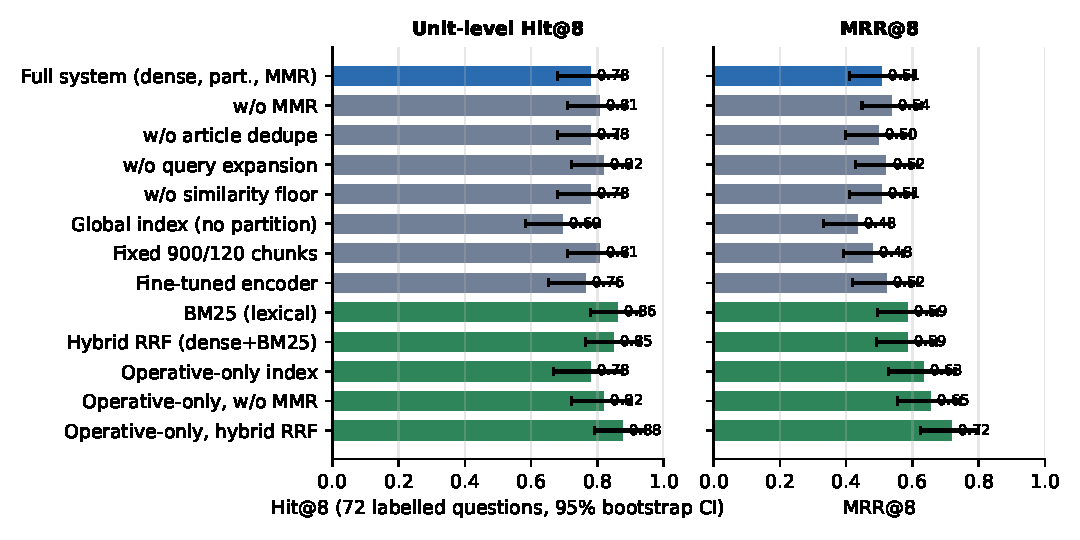
\includegraphics[width=0.95\textwidth]{retrieval_ablation.pdf}
\caption{Unit-level Hit@8 and MRR@8 for every configuration (error bars: 95\% bootstrap CI over questions). Blue: deployed system; grey: ablations and alternative components; green: lexical and error-analysis-driven variants.}
\label{fig:ablation}
\end{figure*}

Table~\ref{tab:retrieval} and Fig.~\ref{fig:ablation} give the main result. The deployed retriever finds a chunk from the governing provision within the top~8 for 78\% of questions \ci{68}{88}, and ranks it first for roughly half of them (MRR $0.51$). Per category (Fig.~\ref{fig:bycat}) it is strong on GDPR (0.85), CCPA (1.0; seven chunks) and cross-jurisdiction questions (1.0), weaker on DPDP (0.68) and poor on ambiguous questions (0.20).

\begin{figure}[t]
\centering
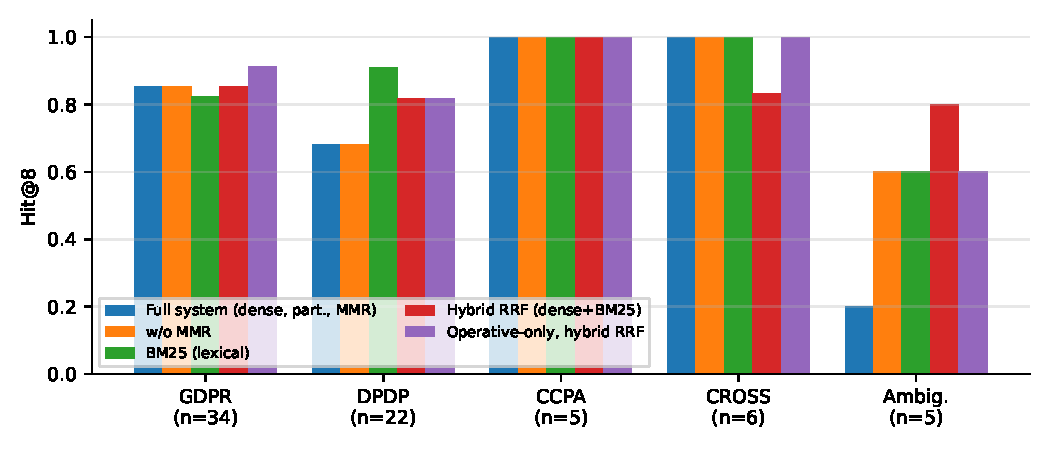
\includegraphics[width=\columnwidth]{retrieval_by_category.pdf}
\caption{Hit@8 by question category for selected configurations.}
\label{fig:bycat}
\end{figure}

\textbf{Ablations.} Removing MMR raises Hit@4 from 0.64 to 0.76 and Hit@8 by $+0.03$ \ci{-0.04}{+0.10}: on this corpus MMR trades away relevant chunks for diversity among a small candidate pool, so the first draft's claim that MMR improved recall is not supported. Removing query expansion gives $+0.04$ \ci{0.00}{+0.10} at lower latency; the regex-triggered sub-queries pull in generic passages. Removing the similarity floor changes nothing on the labelled questions---the floor of 0.22 never binds---and only one question (A01) returned zero passages because of it. Article-level de-duplication has no net effect on Hit@8 because it operates on the wrong keys for most chunks (Section~\ref{sec:benchmark}). Jurisdiction partitioning is the one deployed design choice with a measurable benefit: searching a single global index costs $-0.08$ Hit@8 \ci{-0.15}{-0.03} and drops jurisdiction precision from 0.99 to 0.57, i.e.\ nearly half of the returned passages would come from a regime the user did not ask about.

\textbf{Baselines.} BM25 over the same chunks reaches Hit@8 $=0.86$ and MRR $0.59$, better than the dense retriever on every category except GDPR, at one tenth of the latency. Reciprocal-rank fusion of the two is comparable (0.85/0.59) and has the best precision@8. Both lexical variants, however, have poor cross-jurisdiction coverage (0.58 vs.\ 0.81) because their raw scores are not comparable across indices and one regime crowds out the others in the merged list; a per-jurisdiction quota would be required to deploy them. Fixed 900/120-character windows perform about as well as hierarchy-aware chunks (0.81 vs.\ 0.78), so the chunker's benefit is reproducible citations and readable excerpts rather than retrieval quality. The domain-adapted encoder (146 training pairs, two epochs) does not help ($-0.01$).

\textbf{Error analysis and a better configuration.} Thirteen of the sixteen misses are GDPR or DPDP questions whose top results are recital or definition text: 51\% of the GDPR index is recitals, and recitals discuss the same concepts as the articles in more generic language. Dropping the 308 recital chunks from the index leaves Hit@8 unchanged but raises MRR from 0.51 to 0.63, and combining the operative-only index with hybrid fusion gives the best configuration we found: Hit@4 $=0.86$, Hit@8 $=0.88$ \ci{0.79}{0.94}, MRR $0.72$, $\Delta$Hit@8 $=+0.10$ \ci{+0.01}{+0.19} against the deployed system. We report it as the recommended default rather than as a contribution: it is BM25 plus a filter.

\textbf{Out-of-scope questions.} All configurations return passages for all eight out-of-scope questions (the floor does not help), with mean top similarity 0.46 versus 0.68 for in-scope questions; the 0.50 low-confidence flag (Section~\ref{sec:batch}) fires for five of the eight. The generation stage, not retrieval, therefore has to carry refusal for these cases (Section~\ref{sec:generation}).

\subsection{Batch sanity check at the 0.50 operating point}
\label{sec:batch}
Before the ablations, a batch run over five GDPR questions with $k=6$ and a relevance threshold of 0.50 was used to pick the low-confidence threshold (Fig.~\ref{fig:batch}). All 30 retrieved chunks scored between 0.60 and 0.90 (per-question means 0.65--0.81), so the 0.50 threshold never removed an in-scope result; against the out-of-scope questions above it fires for 5/8. The risk heuristic rated 29 of the 30 chunks low and none high. We include the run because its settings differ from the benchmark ($k=6$, threshold $0.50$) and were previously reported without that context.

\begin{figure}[t]
\centering
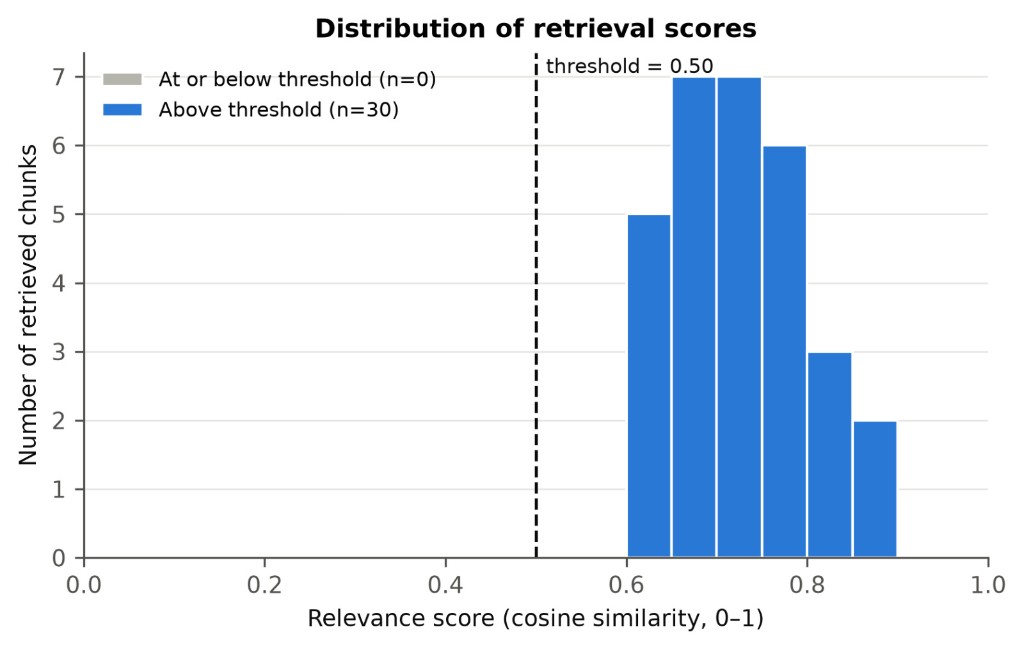
\includegraphics[width=0.49\columnwidth]{batch_score_distribution.jpg}\hfill
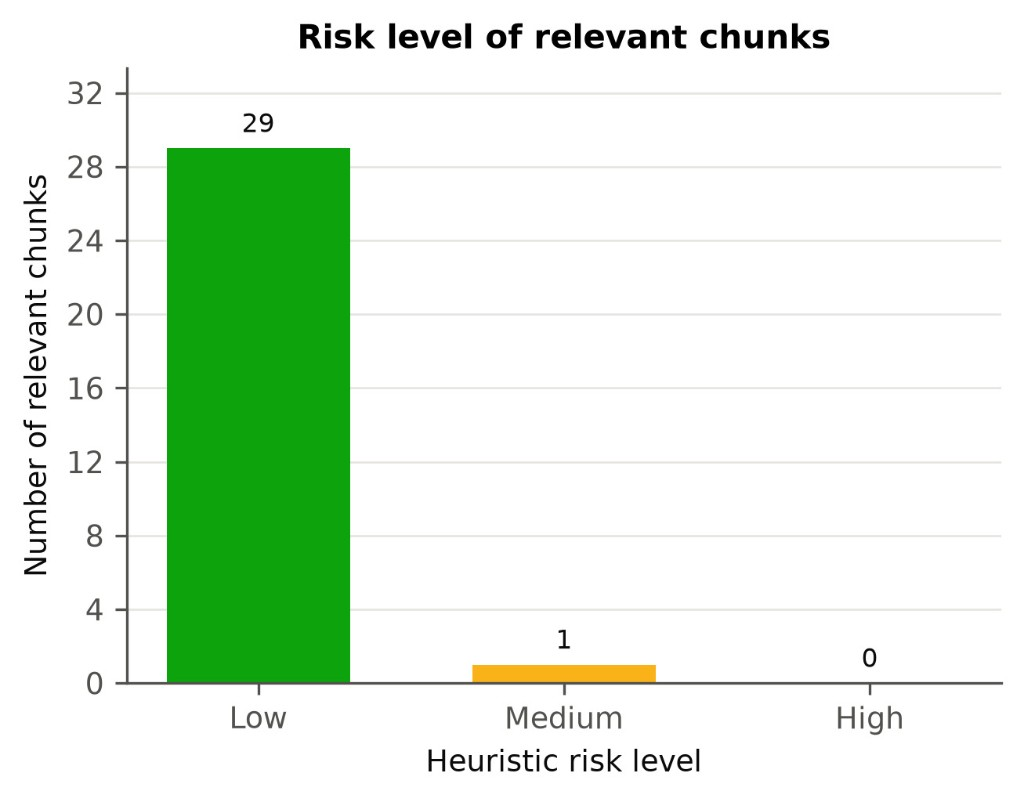
\includegraphics[width=0.49\columnwidth]{batch_risk_levels.jpg}\\[2pt]
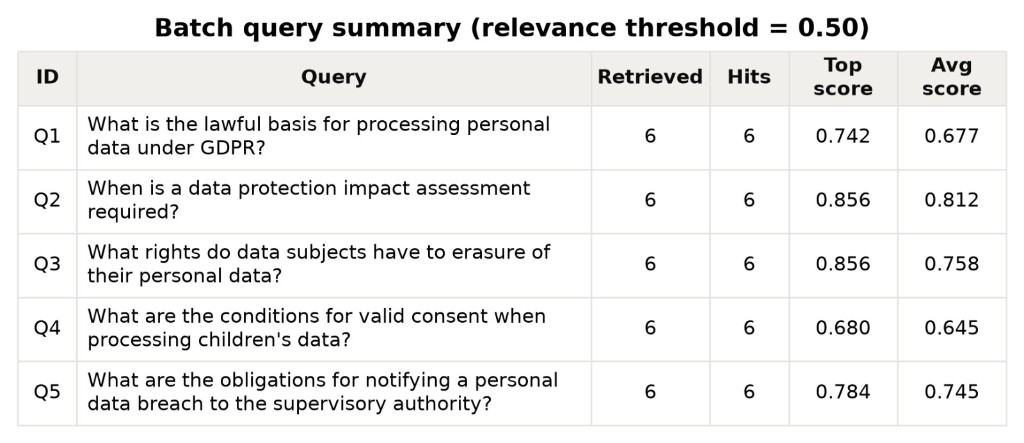
\includegraphics[width=\columnwidth]{batch_summary_table.jpg}
\caption{Batch run on five GDPR questions ($k=6$, threshold $0.50$). Left: distribution of cosine scores of the 30 retrieved chunks; right: heuristic risk levels; bottom: per-question summary.}
\label{fig:batch}
\end{figure}

\section{MMR Latency}
\label{sec:mmr}
The first draft reported that MMR added 468\,ms per query. Selecting 8 of $\approx$18 candidates by MMR requires a few hundred dot products and should take microseconds. Profiling each stage of \texttt{retrieve()} (Fig.~\ref{fig:mmr}) shows that the selection loop takes 0.3\,ms; the cost was the implementation re-encoding every candidate's text with the sentence encoder (110\,ms on this CPU) and re-encoding the query (4\,ms) although both vectors already existed. The fix reads candidate vectors back from the flat FAISS index (\texttt{reconstruct}) and re-uses the primary sub-query vector. Table~\ref{tab:mmr} shows the end-to-end effect: MMR now costs 0.1\,ms, and the selections are identical to the re-encoding implementation on all 40 questions where MMR was active. The ``MMR trade-off'' of the first draft was an artefact; the remaining question is only whether MMR helps retrieval, and Section~\ref{sec:retrieval} shows it does not.

\begin{figure}[t]
\centering
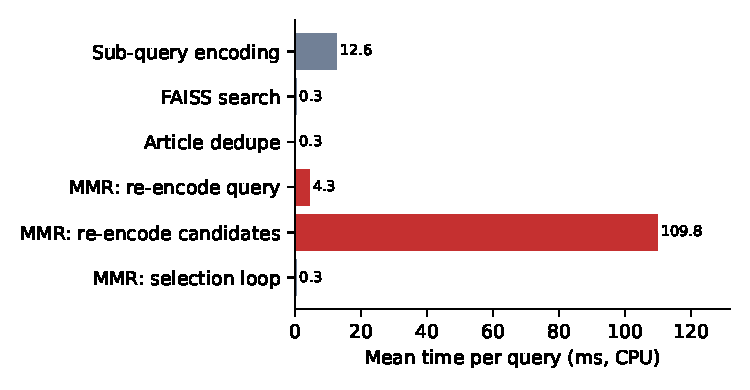
\includegraphics[width=\columnwidth]{mmr_profile.pdf}
\caption{Mean per-query time of each retrieval stage in the original implementation (80 questions, CPU). Red bars are redundant encoder calls.}
\label{fig:mmr}
\end{figure}

\begin{table}[t]
\centering
\caption{End-to-end retrieval latency per question (mean $\pm$ SD over three passes of 80 questions, CPU).}
\label{tab:mmr}
\small
\begin{tabular}{@{}lcc@{}}
\toprule
Retriever & MMR on (ms) & MMR off (ms) \\
\midrule
Original (re-embeds candidates) & 125.8 $\pm$ 1.2 & 10.7 $\pm$ 0.1 \\
Fixed (reads vectors from index) & 10.9 $\pm$ 0.0 & 10.8 $\pm$ 0.2 \\
\bottomrule
\end{tabular}
\end{table}

\section{Generation and Refusals}
\label{sec:generation}

\begin{table}[t]
\centering
\caption{Citation-bound generation on the 72 labelled questions ($k=4$). ``Original'' re-scores the logged outputs of one 3B run with the first draft's validator; ``fixed'' runs use the validator of Section~\ref{sec:validator}. Latency includes the retry.}
\label{tab:gen}
\scriptsize
\setlength{\tabcolsep}{3pt}
\resizebox{\columnwidth}{!}{\begin{tabular}{@{}llcccc@{}}
\toprule
Model & Validator & Runs & Answer rate (\%) & Refusal (\%) & s/question \\
\midrule
Llama 3.2 3B (Q4) & original (re-scored) & 1 & 47.2 & 52.8 & 5.7 \\
Llama 3.2 3B (Q4) & fixed & 3 & 88.4 $\pm$ 2.1 & 11.6 & 2.9 \\
Llama 3.1 8B (Q4) & fixed & 2 & 93.1 $\pm$ 2.0 & 6.9 & 4.6 \\
\bottomrule
\end{tabular}}
\end{table}

\begin{figure}[t]
\centering
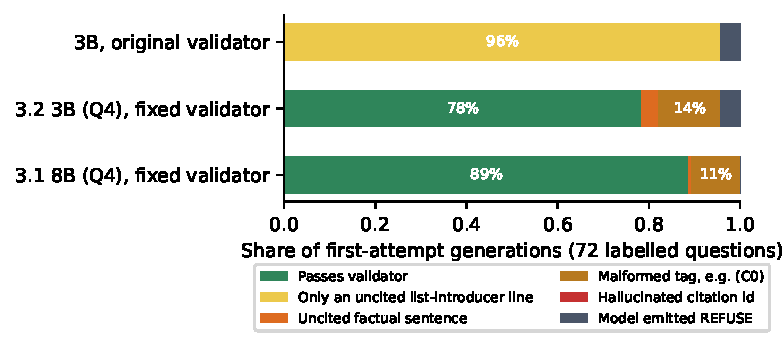
\includegraphics[width=\columnwidth]{refusal_diagnosis.pdf}
\caption{What happens to the model's \emph{first} attempt. Under the original validator almost every 3B answer was rejected for a single uncited line that was not a factual claim.}
\label{fig:refusal}
\end{figure}

\subsection{Diagnosis}
With the first draft's validator the 3B model answers 47\% of the labelled questions and refuses 53\% (Table~\ref{tab:gen}); on the first draft's six cases the same mechanism produced the 40\% figure. Fig.~\ref{fig:refusal} attributes every first-attempt rejection. The model emitted \texttt{REFUSE} for 3 of 72 questions (4\%). It cited an identifier outside the allowed set in none. In 68 of 72 cases (94\%) the rejection was caused by a single line: the model opened with ``Here are 3--6 bullet points summarizing \ldots:'' and the validator, which required every line of at least twelve characters to carry a tag, counted the introducer as an uncited claim. The strict re-prompt produced the same introducer about half the time, which is where the refusals came from. Two further artefacts surfaced: the sentence splitter broke after enumerators and abbreviations (``G. RIGHT TO NON-DISCRIMINATION'', ``Art. 9''), producing tag-less fragments, and the 3B model sometimes wrote \texttt{(C0)} instead of \texttt{[C0]}. The refusals were thus a pipeline property, not a knowledge ceiling of the 3B model.

\subsection{Validator fix and ablation}
\label{sec:validator}
We changed two rules and nothing else: (i) a line that ends with a colon and carries no tag is a list introducer and is not a claim; (ii) sentence splitting does not break after single-letter or numeric enumerators and common legal abbreviations. The per-sentence requirement itself is unchanged, and malformed tags still fail. Table~\ref{tab:validator} re-scores the logged 3B outputs under each rule separately: the introducer rule alone moves the first-attempt pass rate from 0\% to 74\% and the loop refusal rate from 53\% to 13\%; the splitter rule adds one more question. Checking only that cited identifiers are valid---the first draft's ``citation precision''---would have passed 85\% of first attempts, which shows how little that metric measured. The same fix repairs the template baseline, which failed on CCPA excerpts for the splitter reason.

\begin{table}[t]
\centering
\caption{Validator ablation, re-scoring one logged 3B run (72 labelled questions).}
\label{tab:validator}
\scriptsize
\setlength{\tabcolsep}{3pt}
\resizebox{\columnwidth}{!}{\begin{tabular}{@{}lcc@{}}
\toprule
Validator variant & First-attempt pass (\%) & Loop refusal (\%) \\
\midrule
Valid citation ids only (no per-sentence rule) & 84.5 & -- \\
Per-sentence, original & 0.0 & 52.8 \\
\quad + abbreviation-aware sentence splitter & 0.0 & 51.4 \\
\quad + ignore list-introducer lines & 73.6 & 12.5 \\
\quad + both (deployed) & 75.0 & 11.1 \\
\bottomrule
\end{tabular}}
\end{table}

\subsection{Re-run with the fixed validator and a larger model}
% Prose fragment with numbers taken from results/generation_*fixed*.json (edit if the runs are repeated).
With the fixed validator in the loop, the 3B model answers $88.4\pm2.1\%$ of the labelled questions over three runs (refusal $11.6\%$) and the 8B model $93.1\pm2.0\%$ over two runs (refusal $6.9\%$; Table~\ref{tab:gen}). The first attempt now passes for 77\% (3B) and 88\% (8B) of questions; the remaining first-attempt failures are almost all \emph{malformed tags}---the model writes \texttt{(C0)} or a bare \texttt{C0} instead of \texttt{[C0]} (13\% of 3B and 10\% of 8B first attempts)---and the strict retry repairs most of them. Hallucinated citation identifiers did not occur in any of the 360 labelled-question generations across the five runs. The 3B model emitted \texttt{REFUSE} for the same three in-scope questions in every run (D02 on tracking and targeted advertising to children, D19 on penalties for inadequate security safeguards, and the ambiguous bundled-consent question A04); for D02 and A04 the retriever had not returned the governing provision, so these are correct refusals; for D19 Section~33 was the top passage and the refusal is a false negative of the model. The 8B model never emitted \texttt{REFUSE} on an in-scope question; its few refusals (D15, C05 in both runs) are validator failures after two malformed attempts.

By category (Table~\ref{tab:refcat}) the two DPDP cases that dominated the first draft's refusals no longer stand out: 3B refusal is 15\% on DPDP versus 9\% on GDPR, and 8B refusal is 9\% versus 1\%. Ambiguous questions are refused most often by both models (40\% and 20\%), which is the desired direction. On the eight out-of-scope questions the picture reverses: the 3B model refuses 62\% of them, always by emitting \texttt{REFUSE} at the first attempt, whereas the 8B model refuses only 44\%, and never by saying \texttt{REFUSE}---its refusals are validator failures. The larger model is better at following the citation format and worse at declining questions the evidence cannot answer, so the model upgrade reduces in-scope refusals at the cost of answering out-of-scope questions from loosely related passages (e.g.\ an LGPD question answered from Article~45 adequacy text). A dedicated relevance check before generation, rather than a larger model, is the appropriate fix for that failure.

End-to-end latency per question (retrieval, generation and retry) is $2.9$\,s for the 3B model and $4.6$\,s for the 8B model on the RTX~5060 laptop GPU with 4-bit weights; the 15\,s figure in the first draft was reported without hardware details and we could not reproduce it on this machine.


\begin{table}[t]
\centering
\caption{Refusal rate (\%) by category with the fixed validator (mean over runs). For out-of-scope questions refusal is the desired behaviour.}
\label{tab:refcat}
\scriptsize
\setlength{\tabcolsep}{4pt}
\resizebox{\columnwidth}{!}{\begin{tabular}{@{}lcccccc@{}}
\toprule
Model & GDPR & DPDP & CCPA & CROSS & Ambiguous & Negative \\
\midrule
Llama 3.2 3B (Q4) & 9 & 15 & 0 & 0 & 40 & 62 \\
Llama 3.1 8B (Q4) & 1 & 9 & 20 & 8 & 20 & 44 \\
\bottomrule
\end{tabular}}
\end{table}

\section{Faithfulness}
\label{sec:faith}
Citation validity is enforced by construction and says nothing about whether the cited excerpt supports the sentence. Following ALCE~\cite{gao2023alce} we treat every substantive sentence of a validated answer as a claim and score it with an NLI cross-encoder (\texttt{nli-deberta-v3-base}~\cite{he2023debertav3}) against (a) the excerpt(s) it cites and (b) every excerpt in the prompt. A claim is \emph{supported} if entailment is the arg-max label for its best cited excerpt; a claim that is entailed by some excerpt but not by the one it cites is \emph{supported but mis-cited}.

% Prose fragment with numbers taken from results/faithfulness.json and results/spot_check_judgments.json.
Table~\ref{tab:faith} gives the result for the first fixed-validator run of each model; Fig.~\ref{fig:faith} shows the distribution of the entailment probability per claim. The 3B model produced 403 claims over 67 validated answers (6.0 per answer), of which 32.3\% are entailed by the excerpt they cite, 63.5\% are neutral and 4.2\% are contradicted; a further 4.0\% are entailed by some other excerpt in the prompt, i.e.\ supported but mis-cited. No 3B answer had every claim entailed. The 8B model produced shorter answers (5.4 claims per answer) and is markedly better: 50.4\% of claims are entailed by the cited excerpt, 44.1\% are neutral, 5.5\% are contradicted, 3.4\% are mis-cited, and 9.9\% of answers are fully entailed. Support is lowest for both models on the out-of-scope questions they chose to answer (16.7\% and 11.5\% of claims entailed), which is further evidence that those answers should have been refusals. Contradictions are rare; the dominant failure is a \emph{neutral} claim---a sentence whose cited excerpt neither says nor denies it. Given that the validator guarantees every claim carries a tag that resolves to a retrieved excerpt, this is the quantity that ``100\% citation precision'' concealed: a valid citation accompanies a sentence its excerpt actually supports in roughly one case in three for the 3B model and one in two for the 8B model.

The NLI judge is itself uncertain on this material, so one author (not a lawyer) read a stratified sample of 20 claims from the 3B run (8 labelled entailed, 10 neutral, 2 contradicted) with their cited excerpts. The author judged 12 claims supported, 3 partially supported (content supported but modality overstated or a provision number wrong), and 5 unsupported. Of the 8 NLI-entailed claims, 7 were supported and 1 partial; of the 12 NLI-neutral or contradicted claims, 5 were in fact supported---the judge calls \emph{neutral} a claim that paraphrases or compresses the excerpt (e.g.\ listing several lawful bases from Article~6 in one sentence). The NLI figures above are therefore a lower bound on support; a rough extrapolation from this small sample puts the true 3B support rate nearer 50\% than 32\%, and the ranking of the two models is unaffected. The spot check also surfaced a defect that NLI cannot detect: in 4 of the 20 claims the model quotes an Article or Section number that it copied from the excerpt's heading, and the heading was wrong because of the parser problem described in Section~\ref{sec:benchmark}. The excerpt supports the proposition; the cited provision number does not. Correcting the heading field at ingestion is therefore a faithfulness fix as much as a retrieval one. The sample and judgments are in \texttt{results/spot\_check\_judgments.json}.


\begin{table}[t]
\centering
\caption{Claim-level NLI support of validated answers (first fixed-validator run per model).}
\label{tab:faith}
\scriptsize
\setlength{\tabcolsep}{3pt}
\resizebox{\columnwidth}{!}{\begin{tabular}{@{}lcccccc@{}}
\toprule
Model & Answers & Claims & Entailed (cited) & Neutral & Contradicted & Supported, mis-cited \\
\midrule
Llama 3.2 3B & 67 & 403 & 32.3\% & 63.5\% & 4.2\% & 4.0\% \\
Llama 3.1 8B & 71 & 381 & 50.4\% & 44.1\% & 5.5\% & 3.4\% \\
\bottomrule
\end{tabular}}
\end{table}

\begin{figure}[t]
\centering
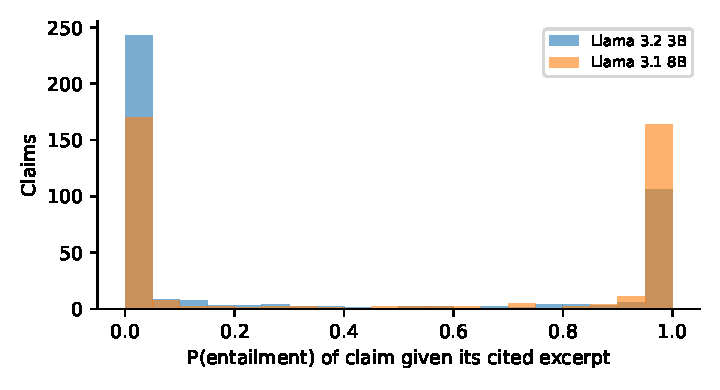
\includegraphics[width=\columnwidth]{faithfulness_hist.pdf}
\caption{Distribution of entailment probability of each claim given its cited excerpt.}
\label{fig:faith}
\end{figure}

\section{The Risk Heuristic, Characterised}
\label{sec:risk}
The first draft presented the risk scorer and stance comparator as a contribution. They have no ground truth, and we did not obtain labelled passages from legal professionals for this revision, so we instead characterise the heuristic over all 712 indexed chunks (Fig.~\ref{fig:risk}). It rates 82\% of the statute low, 9\% medium and 9\% high. The obligation lexicon fires on 42\% of chunks because it matches the word \emph{shall}; prohibition and penalty lexicons fire on 10\% each and the sensitive-data lexicon on 5\%. ``High'' is almost always the conjunction of prohibition and obligation language. 45\% of chunks fire no factor at all, and for those the API reports a \emph{compliance score} of 100, which a reader could mistake for a finding of compliance. The \texttt{without.*consent} pattern matches across a whole chunk and alone explains 6\% of high ratings. Articles that counsel would call restrictive are not reliably high: Article~22 (automated decisions) and DPDP Section~16 (transfers) chunks are rated low. We therefore (i) relabel the component in the interface as a lexical \emph{signal} with its firing factors shown, (ii) stop reporting the 100 score when no factor fires, and (iii) drop the stance comparator from the contribution list. Validating or replacing the heuristic requires at least 30--50 passages labelled by lawyers, which we list as future work.

\begin{figure}[t]
\centering
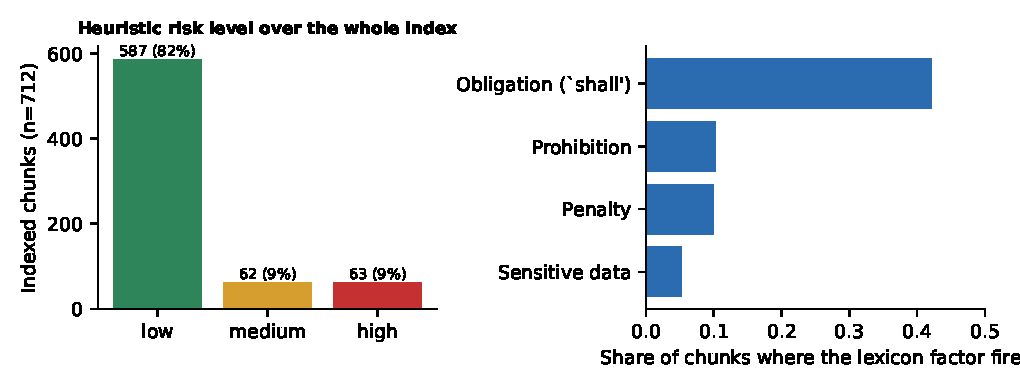
\includegraphics[width=\columnwidth]{risk_distribution.pdf}
\caption{Heuristic risk levels and lexicon firing rates over the whole index.}
\label{fig:risk}
\end{figure}

\section{Limitations}
Our relevance labels are at the level of statutory units and were written by the authors; a lawyer may disagree with some gold assignments, and unit-level hit says nothing about whether the specific paragraph needed was retrieved. The CCPA part of the corpus is a seven-chunk overview page, so CCPA results are not informative about the statute. NLI judges are imperfect on legal register and long premises~\cite{laban2022summac,honovich2022true}; our author spot-check is not a legal review. We evaluated two quantised local models at one temperature; a hosted frontier model would likely change the generation numbers but not the retrieval ones. The benchmark has 72 labelled questions: several differences in Table~\ref{tab:retrieval} have intervals that include zero, and we have described them as such. Finally, the system has not been evaluated by its intended users.

\section{Conclusion}
Treating provenance as a system constraint is cheap to implement and easy to over-claim. Re-evaluating \sys{} with unit-level labels, baselines and confidence intervals reversed several of our own earlier conclusions: keyword checks had passed cases that never retrieved the governing article, MMR cost nothing and helped nothing, the similarity floor was inert, BM25 beat the dense index, and the 3B model's refusals were caused by a validator rule rather than by the model. What survived is the jurisdiction partition, the deterministic citation plumbing, and the refusal mechanism itself, which, once its false positives were removed, refuses out-of-scope questions far more often than in-scope ones. The next steps are the ones we could not do here: relevance and faithfulness labels from legal professionals, an evaluation of the risk display against those labels, and a user study with the compliance teams the system is meant to serve.

\section*{Reproducibility}
The repository contains the index, the 80-question benchmark (\texttt{paper/experiments/questions.json}), every script used here (\texttt{build\_gold.py}, \texttt{run\_retrieval.py}, \texttt{profile\_mmr.py}, \texttt{run\_generation.py}, \texttt{rediagnose.py}, \texttt{run\_faithfulness.py}, \texttt{run\_risk\_analysis.py}, \texttt{make\_figures.py}) and the raw JSON results, including every LLM output. \texttt{scripts/run\_benchmarks.py} runs the original six-case suite.

\bibliographystyle{IEEEtran}
\bibliography{refs}

\appendices

\section{Generation prompt}
\label{app:prompt}
System message (the strict re-prompt appends the sentence in brackets):
\begin{lstlisting}
You are a compliance research assistant. Answer ONLY using the evidence blocks below. Every factual sentence MUST end with one or more citation tags like [C0] drawn ONLY from: C0, C1, C2, C3. Do not invent citations. Do not give legal advice - summarize retrieved evidence. If evidence is insufficient, reply with exactly: REFUSE
[STRICT MODE: Each bullet point must contain at least one [C#] tag. Do not write any sentence without a citation tag from the allowed list.]
\end{lstlisting}
User message:
\begin{lstlisting}
Query: <question>
Product feature: <product context>

Evidence:
[C0] (GDPR - Regulation (EU) 2016/679 (GDPR) | Article 33)
<excerpt, <= 1200 chars>

[C1] ...

Write 3-6 bullet points. Each bullet must cite at least one [C#] tag.
\end{lstlisting}
Decoding: temperature 0.1, at most 800 new tokens, one strict retry.

\section{Deployment stack}
\label{app:stack}
\begin{table}[h]
\centering
\scriptsize
\begin{tabular}{@{}ll@{}}
\toprule
Layer & Components \\
\midrule
Front end & React 18, TypeScript, Vite, Tailwind \\
API & FastAPI, Pydantic v2, JWT (HS256), per-route rate limits (10--30/min) \\
Retrieval & sentence-transformers 5.5, faiss-cpu 1.13 (one \texttt{IndexFlatIP} per jurisdiction) \\
Generation & Ollama (Llama 3.2 3B / Llama 3.1 8B, Q4\_K\_M); optional OpenAI-compatible endpoint; template fallback \\
Storage & PostgreSQL + SQLAlchemy (documents, sections, chunks, analysis history) \\
Parsing & PyMuPDF, BeautifulSoup \\
\bottomrule
\end{tabular}
\end{table}

\section{Per-question results}
\label{app:perq}
Tables~\ref{tab:perq1} and~\ref{tab:perq2} list every question with its gold unit(s), unit-level Hit@8 for the deployed system (Sys), BM25 and the operative-only hybrid (Op-hyb), and the generation outcome of the first fixed-validator run of each model: A1 = answered at first attempt, A2 = answered after the strict retry, R = model emitted \texttt{REFUSE}, V = refused after two validator failures, N = no passage above the floor.

\begin{table*}[p]
\centering
\caption{Per-question results (1/2).}
\label{tab:perq1}
\tiny
\setlength{\tabcolsep}{3pt}
\begin{tabular}{@{}llp{3.1cm}cccc c@{}}
\toprule
ID & Question & Gold unit(s) & Sys & BM25 & Op-hyb & 3B & 8B \\
\midrule
G01 & What is the lawful basis for processing personal data under GDPR? & Art.\,6 & 1 & 1 & 1 & A1 & A1 \\
G02 & What conditions must consent satisfy to be valid, and can it be withdrawn? & Art.\,7 & 1 & 1 & 1 & A1 & A1 \\
G03 & At what age can a child give consent to an online service without a parent? & Art.\,8 & 1 & 1 & 1 & A1 & V \\
G04 & Can we process biometric health data without explicit consent? & Art.\,9 & 0 & 1 & 1 & A1 & A1 \\
G05 & What rights do data subjects have to erasure of their personal data? & Art.\,17 & 1 & 0 & 1 & A1 & A1 \\
G06 & What information must a privacy notice contain when data is collected direc... & Art.\,13 & 0 & 1 & 1 & V & A1 \\
G07 & What information must be provided when personal data was not obtained from... & Art.\,14 & 1 & 1 & 1 & A2 & A1 \\
G08 & What is the right of access and what must the controller provide to the dat... & Art.\,15 & 1 & 0 & 1 & A1 & A1 \\
G09 & How quickly must a controller respond to a data subject request and can it... & Art.\,12 & 1 & 1 & 1 & A1 & A1 \\
G10 & What does the right to data portability require? & Art.\,20 & 1 & 1 & 1 & A1 & A1 \\
G11 & Can a data subject object to processing for direct marketing purposes? & Art.\,21 & 1 & 1 & 1 & V & A1 \\
G12 & What rules apply to automated decision-making and profiling? & Art.\,22 & 1 & 1 & 1 & A1 & A1 \\
G13 & What must a contract between a controller and a processor contain? & Art.\,28 & 1 & 1 & 1 & A1 & A1 \\
G14 & Must we keep records of processing activities and what must they contain? & Art.\,30 & 1 & 1 & 1 & A1 & A1 \\
G15 & What security measures are required for processing personal data? & Art.\,32 & 0 & 1 & 1 & A1 & A1 \\
G16 & What are the obligations for notifying a personal data breach to the superv... & Art.\,33 & 1 & 1 & 1 & A1 & A1 \\
G17 & When must a personal data breach be communicated to the affected individuals? & Art.\,34 & 1 & 1 & 1 & A1 & A1 \\
G18 & When is a data protection impact assessment required? & Art.\,35 & 1 & 1 & 1 & A1 & A1 \\
G19 & When must a data protection officer be designated? & Art.\,37 & 1 & 1 & 1 & A1 & A1 \\
G20 & Under what conditions can personal data be transferred to a third country o... & Art.\,44, Art.\,45, Art.\,46 & 1 & 1 & 1 & A1 & A1 \\
G21 & What are standard contractual clauses and binding corporate rules used for? & Art.\,46, Art.\,47 & 1 & 0 & 1 & A1 & A1 \\
G22 & What derogations allow a transfer without an adequacy decision or appropria... & Art.\,49 & 1 & 1 & 1 & V & A2 \\
G23 & What are the maximum administrative fines for infringing the regulation? & Art.\,83 & 1 & 1 & 1 & A1 & A1 \\
G24 & What does the principle of data minimisation require? & Art.\,5 & 1 & 1 & 1 & A2 & A1 \\
G25 & How long may personal data be stored under the storage limitation principle? & Art.\,5 & 1 & 1 & 1 & A1 & A1 \\
G26 & Does the regulation apply to a company established outside the EU that offe... & Art.\,3 & 1 & 0 & 0 & A1 & A2 \\
G27 & What does data protection by design and by default require? & Art.\,25 & 0 & 0 & 0 & A1 & A1 \\
G28 & What is required when two organisations jointly determine the purposes and... & Art.\,26 & 0 & 1 & 1 & A2 & A1 \\
G29 & Where can a data subject lodge a complaint about how their data is processed? & Art.\,77 & 1 & 1 & 1 & A1 & A1 \\
G30 & Can a person claim compensation for damage caused by an infringement? & Art.\,82 & 1 & 1 & 1 & A1 & A1 \\
G31 & What is the right to rectification of inaccurate personal data? & Art.\,16 & 1 & 1 & 1 & A1 & A1 \\
G32 & When can a data subject obtain restriction of processing? & Art.\,18 & 1 & 1 & 1 & A1 & A1 \\
G33 & Can we process personal data relating to criminal convictions and offences? & Art.\,10 & 1 & 1 & 1 & A1 & A1 \\
G34 & Can the controller rely on legitimate interests to process personal data? & Art.\,6 & 1 & 0 & 0 & A1 & A1 \\
D01 & What consent is required to process personal data of children? & S.\,9 & 1 & 1 & 1 & A1 & A1 \\
D02 & Can we track children's behaviour or show them targeted advertising? & S.\,9 & 0 & 1 & 1 & R & A2 \\
D03 & What must the notice given to a Data Principal contain before seeking consent? & S.\,5 & 0 & 1 & 1 & A1 & V \\
D04 & What are the characteristics of valid consent under the DPDP Act? & S.\,6 & 1 & 1 & 1 & A1 & A1 \\
D05 & Can a Data Principal withdraw consent and what happens after withdrawal? & S.\,6 & 1 & 1 & 1 & A1 & A1 \\
D06 & What is a Consent Manager and what does it do? & S.\,2, S.\,6 & 1 & 1 & 1 & A1 & A1 \\
\bottomrule
\end{tabular}
\end{table*}

\begin{table*}[p]
\centering
\caption{Per-question results (2/2).}
\label{tab:perq2}
\tiny
\setlength{\tabcolsep}{3pt}
\begin{tabular}{@{}llp{3.1cm}cccc c@{}}
\toprule
ID & Question & Gold unit(s) & Sys & BM25 & Op-hyb & 3B & 8B \\
\midrule
D07 & When can personal data be processed without consent for certain legitimate... & S.\,7 & 0 & 1 & 1 & A1 & A1 \\
D08 & What are the obligations of a data fiduciary under DPDP? & S.\,8 & 1 & 1 & 1 & V & V \\
D09 & What must a Data Fiduciary do when a personal data breach occurs? & S.\,8 & 1 & 1 & 1 & A1 & A1 \\
D10 & When must a Data Fiduciary erase personal data? & S.\,8, S.\,12 & 1 & 1 & 1 & A1 & A1 \\
D11 & What additional obligations apply to a Significant Data Fiduciary? & S.\,10 & 1 & 1 & 1 & A2 & A1 \\
D12 & What information can a Data Principal request access to? & S.\,11 & 0 & 1 & 0 & A2 & A1 \\
D13 & What are the rights to correction and erasure of personal data? & S.\,12 & 1 & 1 & 1 & A2 & A1 \\
D14 & What grievance redressal mechanism must be available to Data Principals? & S.\,13, S.\,8 & 1 & 1 & 1 & A1 & A1 \\
D15 & Can a Data Principal nominate another person to exercise their rights? & S.\,14 & 1 & 1 & 1 & A2 & V \\
D16 & What duties does the Act impose on Data Principals themselves? & S.\,15 & 0 & 0 & 0 & A1 & A1 \\
D17 & Can personal data be transferred outside India? & S.\,16 & 1 & 1 & 1 & A1 & A1 \\
D18 & Which processing activities are exempt from the Act's obligations? & S.\,17 & 1 & 1 & 1 & A1 & A1 \\
D19 & What penalties apply for failing to take reasonable security safeguards? & S.\,33, Schedule & 1 & 1 & 1 & R & A1 \\
D20 & What powers and functions does the Data Protection Board of India have? & S.\,27 & 0 & 1 & 0 & A2 & A1 \\
D21 & Does the Act apply to processing of personal data outside the territory of... & S.\,3 & 1 & 1 & 1 & A1 & A1 \\
D22 & On what grounds may a person process the personal data of a Data Principal? & S.\,4 & 0 & 0 & 0 & A1 & A1 \\
C01 & Can consumers limit use of sensitive personal information like geolocation? & limit\_sensitive\_pi & 1 & 1 & 1 & A1 & A1 \\
C02 & What privacy rights do California consumers have under the CCPA? & right\_to\_know, right\_to\_delete, opt\_out\_sale & 1 & 1 & 1 & A1 & A1 \\
C03 & Can a business charge a different price to a consumer who exercised their C... & non\_discrimination, financial\_incentive & 1 & 1 & 1 & A1 & A1 \\
C04 & Can a consumer opt out of the sale or sharing of their personal information? & opt\_out\_sale & 1 & 1 & 1 & A1 & A1 \\
C05 & Can consumers request deletion of the personal information a business holds... & right\_to\_delete & 1 & 1 & 1 & A2 & V \\
X01 & What are user rights to delete or erase personal data? & Art.\,17 (GDPR); S.\,12 (DPDP); right\_to\_delete (CCPA) & 1 & 1 & 1 & A2 & A1 \\
X02 & What consent is required to process children's personal data? & Art.\,8 (GDPR); S.\,9 (DPDP) & 1 & 1 & 1 & A1 & A2 \\
X03 & What are the obligations to notify a personal data breach? & Art.\,33, Art.\,34 (GDPR); S.\,8 (DPDP) & 1 & 1 & 1 & A1 & A1 \\
X04 & What rights of access to their personal data do individuals have? & Art.\,15 (GDPR); S.\,11 (DPDP); right\_to\_know (CCPA) & 1 & 1 & 1 & A1 & A1 \\
X05 & What penalties can be imposed for non-compliance? & Art.\,83 (GDPR); S.\,33, Schedule (DPDP) & 1 & 1 & 1 & A1 & A1 \\
X06 & Can personal data be transferred to another country? & Art.\,44, Art.\,45, Art.\,46 (GDPR); S.\,16 (DPDP) & 1 & 1 & 1 & A1 & A1 \\
A01 & Can we use email addresses collected for order confirmations to send market... & Art.\,5, Art.\,6, Art.\,21 & 0 & 1 & 1 & N & N \\
A02 & We want to keep user activity logs for ten years. Is that allowed? & Art.\,5 & 1 & 0 & 1 & A1 & A1 \\
A03 & A user asked us to delete their account but we must keep invoices for tax l... & Art.\,17 & 0 & 0 & 0 & A1 & A1 \\
A04 & Is it acceptable to use a single checkbox for terms of service and marketin... & Art.\,7 (GDPR); S.\,6 (DPDP) & 0 & 1 & 1 & R & A1 \\
A05 & Our vendor in India processes EU customer data on our behalf. What do we ne... & Art.\,28, Art.\,44, Art.\,46 & 0 & 1 & 0 & A1 & A1 \\
N01 & What are the HIPAA requirements for encrypting protected health information? & -- & -- & -- & -- & R & V \\
N02 & What is the corporate tax rate for software companies in Ireland? & -- & -- & -- & -- & R & V \\
N03 & How long must a company retain payroll records under India's Companies Act? & -- & -- & -- & -- & R & A1 \\
N04 & What does Brazil's LGPD say about the powers of the national data protectio... & -- & -- & -- & -- & A1 & A1 \\
N05 & What are the cookie banner requirements under the ePrivacy Directive? & -- & -- & -- & -- & A1 & A1 \\
N06 & Does Section 230 shield platforms from liability for user-generated content? & -- & -- & -- & -- & A1 & A1 \\
N07 & What is the maximum weekly working time under the EU Working Time Directive? & -- & -- & -- & -- & R & V \\
N08 & What are the accessibility requirements for mobile apps under the European... & -- & -- & -- & -- & R & A2 \\
\bottomrule
\end{tabular}
\end{table*}

\end{document}
